\documentclass{standalone}
\usepackage{pgfplots}
\pgfplotsset{compat=1.11}
\begin{document}
% Place the TikZ picture in a figure environment.
%\begin{figure}[htb]
% h: here, t: top, b: bottom, p: page of float
%% https://tex.stackexchange.com/questions/39017/how-to-influence-the-position-of-float-environments-like-figure-and-table-in-lat
%% ! indicates that some restrictions should be ignored (discussed later)
%% h indicates that the float is allowed to be placed inline
%% t indicates that the float is allowed to go into a top area
%% b indicates that the float is allowed to go into a bottom area
%% p indicates the the float is allowed to go on a float page or column area

    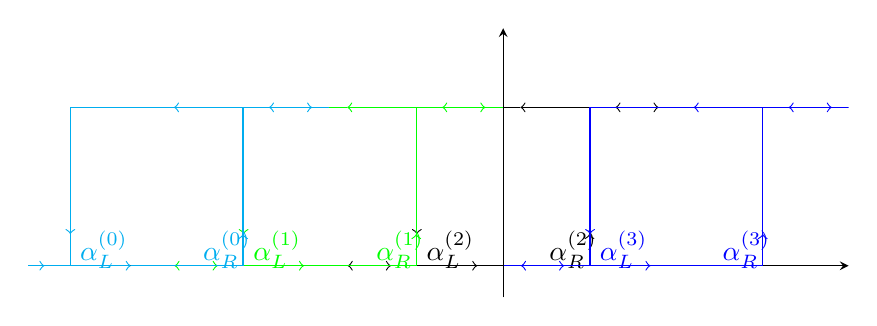
\begin{tikzpicture}
        \begin{axis} [
        width=12cm,height=5cm,
            % xmin=-7.5, xmax=7.5, ymin=-0.5, ymax=1.5, 
            xmin=-5.5, xmax=4.0, ymin=-0.2, ymax=1.5,
            % grid=both,
            ylabel={},
            xlabel=,
            % xtick={-2,-1.5,...,2}, ytick={-2,-1.5,...,2},
            % xticklabel style={font=\tiny, xshift=0.5ex},
            % yticklabel style={font=\tiny, yshift=0.5ex},
            axis line style={->},
            axis x line=middle,
            axis y line=middle,
            ticks=none
        ]
        \addplot+[color=black, dashed, ->, mark=none, domain=-1.3:-1.8] {0};
        \addplot+[color=black, solid, ->, mark=none, domain=-2:-1.3] {0};
        \addplot+[color=black, solid, ->, mark=none, domain=-2:-0.3] {0};
        \addplot+[,color=black, solid, mark=none, domain=-0.3:1] {0};

        \addplot+[color=black, solid, mark=none, ->,domain=1.3:1.8] {+1};

        \addplot+[color=black, solid, mark=none, ->,domain=2:1.3] {+1};
        \addplot+[color=black, solid, mark=none, ->, domain=1.3:0.2] {+1};
        \addplot+[color=black, solid, mark=none, domain=0.2:-1] {+1};

        \draw[color=black, solid, mark=none, ->] (1, 0) -- (1, 0.2);
        \draw[color=black, solid, mark=none] (1, 0) -- (1, +1);

        \draw[color=black, solid, mark=none, ->] (-1, +1) -- (-1, +0.2);
        \draw[color=black, solid, mark=none] (-1, +0.2) -- (-1, 0);

        
        \node[right] at (-1,0.1) {$\alpha^{(2)}_L$};
        \node[left] at (1.2,0.1) {$\alpha^{(2)}_R$};


        %%%%%%%%%%%%%%%%%%%%%%%%%%%%%%%%%%%%%%%%%%%%%%%%%%%%%%
        
        \addplot+[color=blue, dashed, ->, mark=none, domain=-1.3:-1.8][xshift=2.2cm] {0};
        \addplot+[color=blue, solid, ->, mark=none, domain=-2:-1.3][xshift=2.2cm] {0};
        \addplot+[color=blue, solid, ->, mark=none, domain=-2:-0.3][xshift=2.2cm] {0};
        \addplot+[,color=blue, solid, mark=none, domain=-0.3:1][xshift=2.2cm] {0};

        \addplot+[color=blue, solid, mark=none, ->,domain=1.3:1.8][xshift=2.2cm] {+1};

        \addplot+[color=blue, solid, mark=none, ->,domain=2:1.3][xshift=2.2cm] {+1};
        \addplot+[color=blue, solid, mark=none, ->, domain=1.3:0.2][xshift=2.2cm] {+1};
        \addplot+[color=blue, solid, mark=none, domain=0.2:-1][xshift=2.2cm] {+1};

        \draw[color=blue, solid, mark=none, ->][xshift=2.2cm] (1, 0) -- (1, 0.2);
        \draw[color=blue, solid, mark=none][xshift=2.2cm] (1, 0) -- (1, +1);

        \draw[color=blue, solid, mark=none, ->][xshift=2.2cm] (-1, +1) -- (-1, +0.2);
        \draw[color=blue, solid, mark=none][xshift=2.2cm] (-1, +0.2) -- (-1, 0);

        \node[right,color=blue][xshift=2.2cm] at (-1,0.1) {$\alpha^{(3)}_L$};
        \node[left,color=blue][xshift=2.2cm] at (1.2,0.1) {$\alpha^{(3)}_R$};
                

        % %%%%%%%%%%%%%%%%%%%%%%%%%%%%%%%%%%%%%%%%%%%%%%%%%%%
        
        \addplot+[color=green, dashed, ->, mark=none, domain=-1.3:-1.8][xshift=-2.2cm] {0};
        \addplot+[color=green, solid, ->, mark=none, domain=-2:-1.3][xshift=-2.2cm] {0};
        \addplot+[color=green, solid, ->, mark=none, domain=-2:-0.3][xshift=-2.2cm] {0};
        \addplot+[,color=green, solid, mark=none, domain=-0.3:1][xshift=-2.2cm] {0};

        \addplot+[color=green, solid, mark=none, ->,domain=1.3:1.8][xshift=-2.2cm] {+1};

        \addplot+[color=green, solid, mark=none, ->,domain=2:1.3][xshift=-2.2cm] {+1};
        \addplot+[color=green, solid, mark=none, ->, domain=1.3:0.2][xshift=-2.2cm] {+1};
        \addplot+[color=green, solid, mark=none, domain=0.2:-1][xshift=-2.2cm] {+1};

        \draw[color=green, solid, mark=none, ->][xshift=-2.2cm] (1, 0) -- (1, 0.2);
        \draw[color=green, solid, mark=none][xshift=-2.2cm] (1, 0) -- (1, +1);

        \draw[color=green, solid, mark=none, ->][xshift=-2.2cm] (-1, +1) -- (-1, +0.2);
        \draw[color=green, solid, mark=none][xshift=-2.2cm] (-1, +0.2) -- (-1, 0);

        \node[right,color=green][xshift=-2.2cm] at (-1,0.1) {$\alpha^{(1)}_L$};
        \node[left,color=green][xshift=-2.2cm] at (1.2,0.1) {$\alpha^{(1)}_R$};


        %%%%%%%%%%%%%%%%%%%%%%%%%%%%%%%%%%%%%%%%%%%%%%%%%%%%%%
        \addplot+[color=cyan, dashed, ->, mark=none, domain=-1.3:-1.8][xshift=-4.4cm] {0};
        \addplot+[color=cyan, solid, ->, mark=none, domain=-2:-1.3][xshift=-4.4cm] {0};
        \addplot+[color=cyan, solid, ->, mark=none, domain=-2:-0.3][xshift=-4.4cm] {0};
        \addplot+[,color=cyan, solid, mark=none, domain=-0.3:1][xshift=-4.4cm] {0};

        \addplot+[color=cyan, solid, mark=none, ->,domain=1.3:1.8][xshift=-4.4cm] {+1};

        \addplot+[color=cyan, solid, mark=none, ->,domain=2:1.3][xshift=-4.4cm] {+1};
        \addplot+[color=cyan, solid, mark=none, ->, domain=1.3:0.2][xshift=-4.4cm] {+1};
        \addplot+[color=cyan, solid, mark=none, domain=0.2:-1][xshift=-4.4cm] {+1};

        \draw[color=cyan, solid, mark=none, ->][xshift=-4.4cm] (1, 0) -- (1, 0.2);
        \draw[color=cyan, solid, mark=none][xshift=-4.4cm] (1, 0) -- (1, +1);

        \draw[color=cyan, solid, mark=none, ->][xshift=-4.4cm] (-1, +1) -- (-1, +0.2);
        \draw[color=cyan, solid, mark=none][xshift=-4.4cm] (-1, +0.2) -- (-1, 0);

        \node[right,color=cyan][xshift=-4.4cm] at (-1,0.1) {$\alpha^{(0)}_L$};
        \node[left,color=cyan][xshift=-4.4cm] at (1.2,0.1) {$\alpha^{(0)}_R$};

        \end{axis}
    \end{tikzpicture}

\end{document}